\section{Methods}  
    In this section, a brief description of the two simulation methods used for generating a representative hazard scenario is provided, along with their mathematical explanations. Furthermore, a more detailed explanation of MCMC-IS as an adaptive importance sampling method will be presented in this section.
    
    Monte Carlo simulations, a cornerstone of probabilistic modeling, rely on random sampling from specified probability distributions to estimate outcomes and assess uncertainties. The MC method provides a robust framework for exploring a broad range of scenarios, making it particularly valuable when dealing with intricate systems characterized by multiple sources of variability. On the other hand, IS represents a specialized adaptation of the MC method. The fundamental concept behind importance sampling lies in recognizing that certain random input variables or vectors exert a more significant influence on the estimated quantity than others. To mitigate the estimator's variance, it is advantageous to sample these "important" values more frequently, which can be achieved by drawing samples from a biased density function. Subsequently, the simulation results are appropriately weighted to counteract the bias introduced by sampling from this skewed density function.

    Importance sampling techniques involve two primary steps. The first step entails a modification of the initial sampling procedure. To allocate more samples to "important" regions within the sample space, samples are generated from an alternative probability density function (PDF) referred to as an \textit{importance density function}. The second step focuses on rectifying the introduced bias by averaging the outcomes of various samples (realizations) while applying weights associated with the bias. This process ensures that the estimated quantity maintains its true mean, thereby eliminating the distortion caused by the biased sampling approach.
        
    \subsection{Mathematical Expression}
        Let $x$ represent a random variable (or vector) characterized by a (joint) probability density function $p(x)$. The primary objective is to obtain the moments, specifically the mean and variance, of the function $h = f(x)$, where $f$ stands for a specified deterministic function (operator). The mean ($\mu_h$) and variance ($\sigma_h^2$) of $h$ can be expressed as follows:
        $$\mu_h=E[h]=E[f(x)]=\int_\Omega f(x)p(x)dx$$
        $$\sigma_h^2=E{[f(x)-\mu_h]^2}=\int_\Omega[f(x)-\mu_h]^2 p(x)dx = \int_\Omega f^2(x)p(x)dx-\mu^2_h$$
        Where, $\Omega$ is a probability space, $E$ represents statistical expectation and $\mu_h$ and $\sigma_h^2$ are the mean and variance of $h=f(x)$, respectively. 
        
        For the estimation of $\mu_h$ using the MC method, a set of samples $(x_i,\quad i=1,2,…,N)$ is randomly drawn from the density function $p(x)$, and the function mean $(\mu_{MC})$ and variance $(\sigma_{MC}^2)$ are computed as follows:
        $$\mu_{MC}=\frac{1}{N}\sum_{i=1}^{N} f(x_i)$$
        $$\sigma_{MC}^2=\frac{1}{N}\sum_{i=1}^{N}f^2(x_i)-(\frac{1}{N}\sum_{i=1}^{N} f(x_i))^2$$
        Where $\mu_{MC}$ and $\sigma_{MC}^2$ are the mean and variance of $h=f(x)$ estimated using the MC simulation method, respectively.
        
        Sometimes, achieving accurate estimations can be challenging for two primary reasons. Firstly, the original distribution may be difficult to sample from, posing inherent computational complexities. Secondly, accuracy may be compromised when the function $f(x)$ exhibits high values in regions where the probability density function $p(x)$ is low. This latter scenario is particularly prevalent when dealing with natural disasters, where extreme events occur with low probability. In these situations, importance sampling becomes advantageous due to its potential to find accurate estimations more rapidly compared to MC methods. Suppose we draw samples, $(x_i, \quad i=1,2,…,N)$, from an importance density function $q(x)$ rather than the original density function $p(x)$, with $q(x)$ being zero only where $p(x)$ is zero. To correct for the bias and maintain the mean, the original function $f(x)$ is adjusted by introducing a modified function, denoted as $f_q(x)$:
        $$f_q(x)=f(x) w(x)$$
        Where $w(x)=p(x)/q(x)$ is called a weight function. 
        The mean and variance of f(x) can also be written as:
        $$\mu_{IS}=\frac{1}{N} \sum_{i=1}^{N}f(x_i)w(x_i)$$
        $$\sigma_{IS}^2=\frac{1}{N} \sum_{i=1}^N f^2(x_i)w(x_i)-\mu_{IS}^2$$
        Where $\mu_{IS}$ and $\sigma_{IS}^2$ are the mean and variance of $h=f(x)$ estimated using the IS-MC simulation method, respectively. 
        
    \subsection{Selection of Importance Density Functions}
        While Importance Sampling (IS) can often lead to estimates with significantly lower variance compared to their MC counterparts, it's important to note that this reduction in variance is not guaranteed. The effectiveness of IS relies heavily on the selection of an appropriate importance density function, which remains a challenging and non-generalizable process. This issue has been a central focus of numerous papers in the fields of statistics and simulation.
    
        The choice of the importance density function, denoted as $q(x)$, should be made with the dual objectives of minimizing the estimated variance quantity $\sigma_{IS}^2$ and reducing the computational effort required to estimate the mean quantity $\mu_{IS}$. However, directly minimizing the variance of importance sampling estimation as a function of the unknown density function $q(x)$ is a complex task.
        
        Several techniques exist for estimating the importance density function, some of which involve a manual trial-and-error process. In the manual process, $q(x)$ can be selected from the same family distribution as the original distribution $p(x)$ but with different parameters. Notable examples include variance scaling (VS), mean translation (MT), and a combination of both approaches \cite{lu_improved_1988}.
        
        The concepts of MT, VS, and their combination are visually represented in Figure~\ref{fig:IS_techniques}. In this context, $p(x)$ denotes the original density function, $q(x)$ represents the proposed importance density function, and $f(x)$ corresponds to a function within the model under consideration.
        
            \begin{figure}[H]
        \centering
        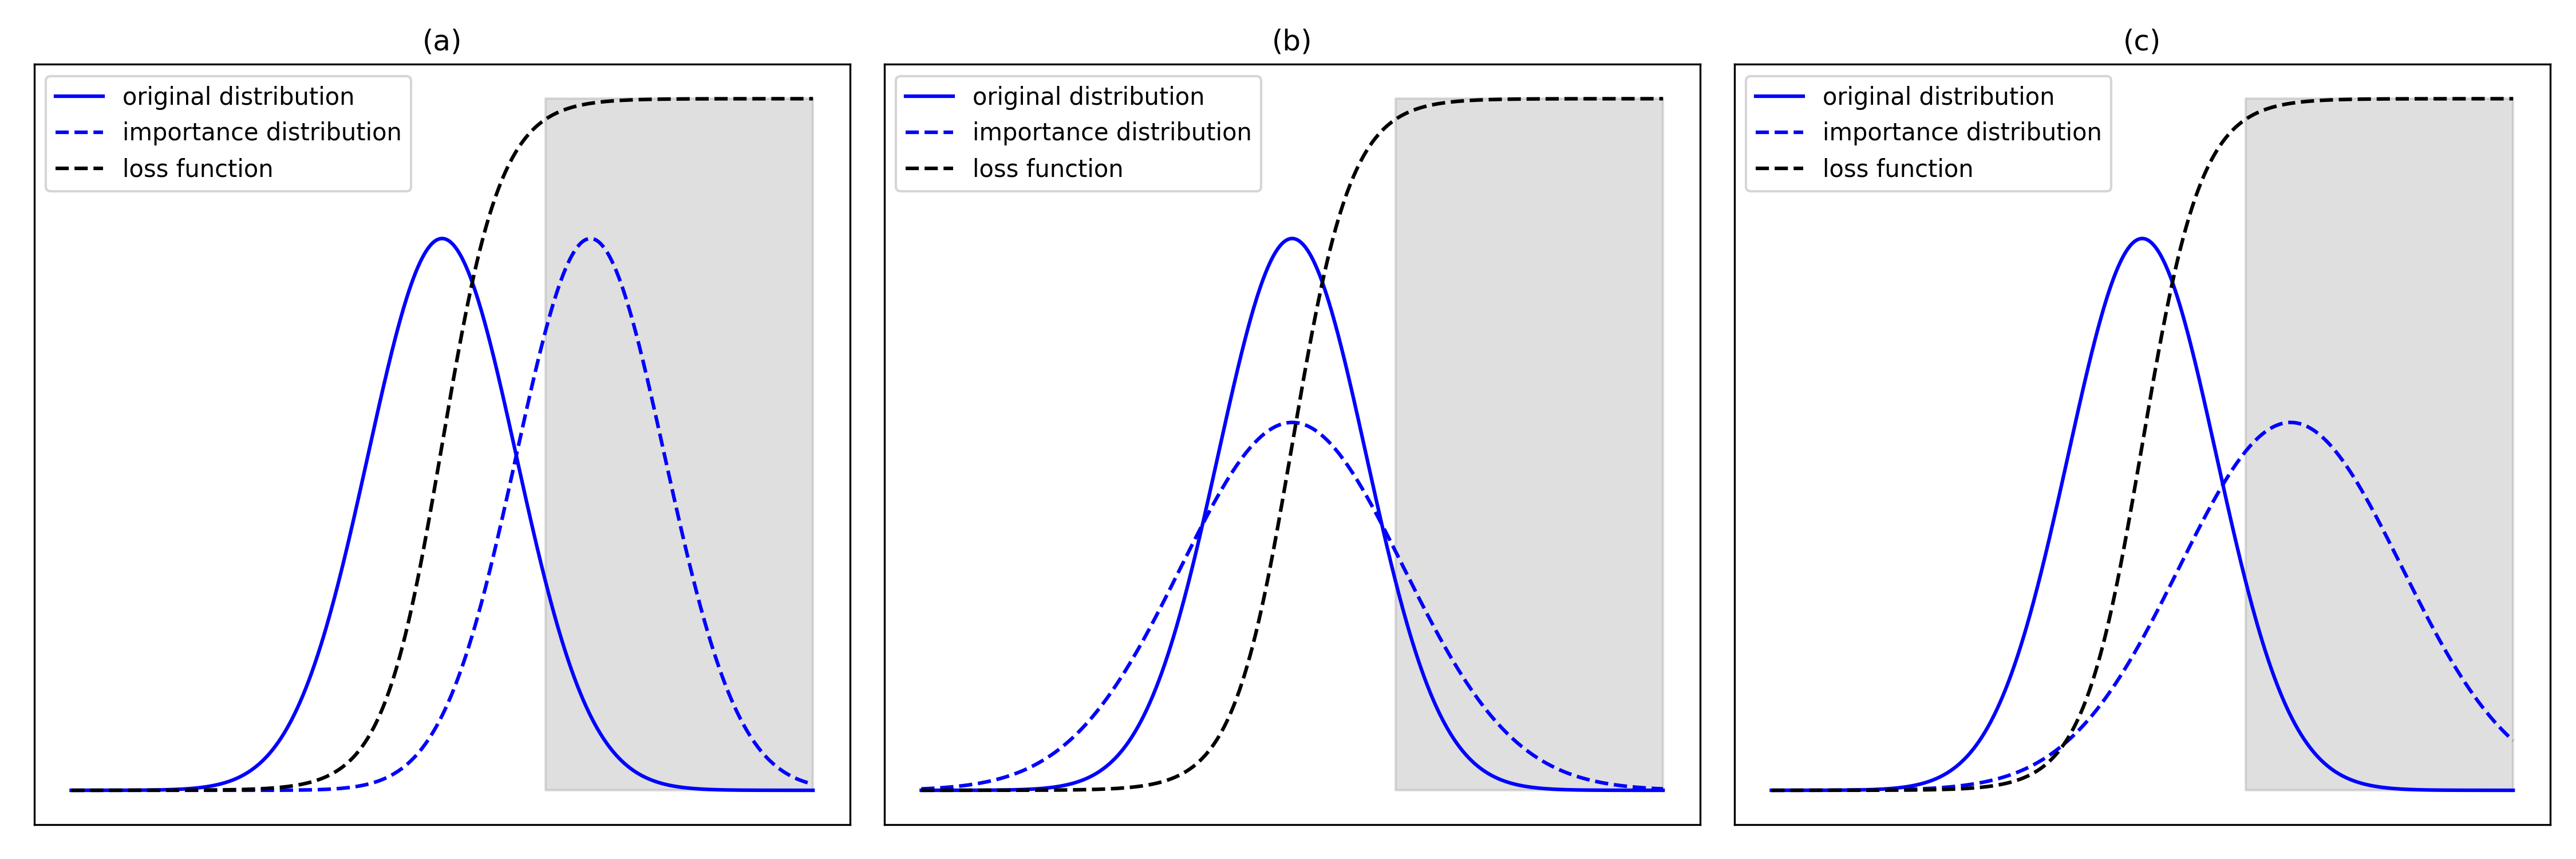
\includegraphics[scale=0.40]{Figures/Images/Methods/IS_techniques.png}
        \caption{Schematic diagrams illustrating (a) mean translation (MT), (b) variance scaling (VS), and (c) their combined application in one dimension. The shaded area denotes the effective probability density employed in importance sampling \protect\cite{lu_improved_1988}}
        \label{fig:IS_techniques}
    \end{figure}
        
        As illustrated in Figure~\ref{fig:IS_techniques}, samples associated with high values of $f(x)$ are situated in the tail region of $p(x)$ where the probability of occurrence is significantly low (indicated by the gray shaded area). In such scenarios, generating more important samples with greater frequency is advantageous. This rationale underlies the mean translation technique, where $q(x)$ aligns with the same probability distribution function as $p(x)$ but with a shifted mean towards the more consequential area, as depicted in Figure~\ref{fig:IS_techniques}a.
        
        Alternatively, another approach to increase sampling frequency is to expand the variance of $p(x)$ to generate more samples in the tail region. This concept is central to the variance scaling technique, as depicted in Figure~\ref{ fig:IS_techniques}b. Furthermore, Figure~\ref{fig:IS_techniques}c showcases the combination of mean translation and variance scaling to optimize importance sampling efficiency.

    \subsection{Markov Chain Monte Carlo Importance Sampling (MCMC-IS) Technique} 
        The manual trial-and-error process for estimating the importance density function can be excessively time-consuming, often requiring multiple iterations to find the optimal importance density parameters. To address this challenge, alternative methods have been proposed for systematically estimating near-optimal importance sampling distributions. One such method is known as MCMC-IS, introduced by Parpas et al \cite{parpas_importance_2015}.

        The MCMC-IS framework comprises three essential steps:
        \begin{enumerate}
            \item Generation of samples from a zero-variance distribution using a Markov Chain Monte Carlo (MCMC) algorithm.
            \item Construction of an approximate zero-variance distribution through Kernel Density Estimation (KDE) algorithm.
            \item Sampling from the approximate zero-variance distribution to produce a lower-variance importance sampling estimate.
        \end{enumerate}

        The first crucial step in the MCMC-IS framework involves the generation of samples using the MCMC method. MCMC is a powerful adaptive sampling technique widely used for approximating complex probability distributions. It operates by iteratively updating the current state based on a proposal distribution, thereby exploring the target distribution of interest. There exist several MCMC algorithms, each tailored to specific scenarios and distributions \cite{gelman_handbook_2010}. In this study, we employ the Metropolis-Hastings algorithm for MCMC sampling. The Metropolis-Hastings algorithm is a widely used choice due to its simplicity of implementation and flexibility \cite{parpas_importance_2015}. It involves generating new samples from a proposal distribution and accepting or rejecting them based on a ratio of the proposed sample's probability to that of the previous sample to ensure the generated samples eventually resemble the target distribution.
        
        However, a significant challenge is picking the right parameters for proposal distribution, like proposal variances, to make the mixing and convergence efficient. To address this challenge, the adaptive Metropolis-Hastings algorithm has emerged as a promising solution, particularly within the MCMC-IS framework. This adaptive technique offers a dynamic approach to adjusting the parameters of MCMC algorithms as they run, effectively enabling the algorithms to "learn" and adapt to better parameter values for more efficient sampling \cite{haario_adaptive_2001}. In this approach, the covariance matrix within the proposal distribution is updated after each chunk of iterations to better reflect the correlations between random variables. The proposal distribution at iteration $n$ is as follows, but for a more detailed explanation, you can refer to \cite{haario_adaptive_2001}:
        $$Q_n(x, \mu)=\mathcal{N}(\mu,{(0.1)}^2I_d/d)\quad \text{for} \quad n\le2d$$
        $$Q_n(x, \mu)=(1-\beta)\mathcal{N}(\mu,{(2.38)}^2\Sigma_n/d) + \beta\mathcal{N}(\mu,{(0.1)}^2I_d/d)\quad \text{for} \quad n>2d$$
        where,
        $Q_n(x, \mu)$ is the proposal distribution at iteration $n$, which generates candidate samples $x$ based on the current state $\mu$;
        $\mathcal{N}(\mu, \sigma^2)$ is the Gaussian distribution with mean $\mu$ and variance $\sigma^2$, used as a building block for constructing the proposal distribution;\\
        $0.1$ is a fixed constant used to set the variance for the proposal distribution when $n$ is less than or equal to $2d$;
        $I_d$ is the identity matrix of dimension $d$;       
        $\beta$ is a weighting factor that blends two Gaussian distributions within the proposal distribution when $n$ is greater than $2d$;      
        $2.38$ is a scaling factor used to adjust the variance of the Gaussian component of the proposal distribution when $n$ is greater than $2d$;        
        $\Sigma_n$ is the covariance matrix updated after each chunk of iterations to better reflect the correlations between random variables.        
        
        Following the generation of MCMC samples, the subsequent step is to construct an approximate zero-variance distribution using the KDE algorithm. KDE is a statistical technique used to estimate the probability density function of a random variable based on the provided samples. KDE relies on two primary parameters: the choice of a kernel function and the bandwidth parameter. The kernel function determines the shape of the kernels placed on each data point, while the bandwidth parameter controls the width of these kernels. The selection of appropriate kernel functions and bandwidth values is essential, as it directly impacts the quality of the estimated importance density.
        

        










